\documentclass[12pt, a4paper]{report}

\usepackage[utf8]{inputenc}
\usepackage[english]{babel}
\usepackage{hyperref}
\hypersetup{
    colorlinks=true,
    linkcolor=blue,
    filecolor=magenta,
    urlcolor=cyan,
}
\usepackage{csquotes}
\usepackage[backend=biber]{biblatex}
\addbibresource{thesis.bib}

\title{
      {Distributed Flow Control and Intelligent Data Transfer in High Performance Computing Networks}\\
      {\large Hochschule Offenburg}
}
\author{Mehdi Sadeghi}

\date{13. Feb 2015}

\begin{document}
\nocite{*} % Everything in bibtex file will appear in bibliography

\maketitle

%\newpage
%\thispagestyle{plain}
%\begin{center}
%\vspace*{\fill}
%\copyright\ Copyright\ 2015\ Mehdi Sadeghi
%\end{center}
%This work is published under the conditions of the
%\textsl{Creative Commons License Attribution--Non-Commercial--No-Derivatives}
%(CC BY-NC-ND)---see \url{http://creativecommons.org/licenses/by-nc-nd/3.0/}.
%\vspace*{\fill}

%\newpage

\chapter*{Declaration}
\noindent
I hereby declare and confirm that this thesis is entirely the result of my own original work. 
Where other sources of information have been used, they have been indicated as such and properly acknowledged. 
I further declare that this or similar work has not been submitted for credit elsewhere.
\\

Offenburg, February 28, 2015

Mehdi Sadeghi


\chapter*{Abstract}
This document contains my master's thesis report, including the problem definiation,
an overview of state of the art, discussions and my suggestions.



\chapter*{Acknowledgement}
Here will come acknowledgement

\tableofcontents

\chapter*{Preface}
\label{cha:preface}

European scientific communities launch many experiments everyday, resulting in huge amounts
of data. Specifically in molecular dynamics and material science fields there are many different
simulation softwares which are being used to accomplish multi-scale modeling tasks. 

These tasks
often involve running multiple simulation programs over the existing datasets or the data which is
produced by other simulation software. It's common to run multiple programs on existing datasets
during one operation to produce the desired results. The order to run simulation software is normally 
defined within scripts written by users. 

Moreover users have to provide the required data manually and copy all required files to a working
directory to submit their job, and they might have to login to different machines to prepare files,
submit the script, monitor the status of the job and finally collect the output files. 
This type of work routine is a common form of workflow management in above mentioned communities.

While simpler and smaller experiments could be handled this way, larger and more complicated experiments
require different solutions. 

Such experiments are the source of many high performance computing (HPC) problems, specially workflow management and data transfer.

%This thesis is an indirect research and development effort in the field of high performance computing (HPC) and scientific simulations.

This thesis is a research and development effort to accomplish such operations in a distributed manner with a 
collective but decentralized approach toward workflow management and to minimize data transfer during such operations.

This work has not been an implementation task nor a purely theoratical work. 
It means that I was not supposed to create an application or develop a software from ground up (even though eventually I did), instead
I have been responsible to study about and define the problem of my client and assist them either with 
finding a suitable solution and helping them to integrate it into their development process or propose a new approach to address their 
needs. My activities include but not limited to analysing the problem, collecting requirements,
studying state of the art software frameworks and related products,
analysing them against the defined requirments, proposing a solution and developing a prototype.

During this thesis an open source prototype application has been developed which is available
online\footnote{https://github.com/mehdisadeghi/konsensus}. The source files
of the current document are also available\footnote{https://github.com/mehdisadeghi/cme-thesis}.
If there are any comments and improvements regarding this document, I
appreciate an email to \textbf{sadeghi@mehdix.org}.

%\begin{center}
%\begin{tabular}{l}
%\nolinkurl{sadeghi@mehdix.org} \\
%Hochschule Offenburg\\
%Mehdi Sadeghi
%\end{tabular}
%\end{center}
\chapter{Introduction}
\label{cha:introduction}
This thesis is an indirect research and development effort in the field of high performance computing (HPC) and scientific simulations.
This has not been an implementation task nor a purely theoratical work. 
It means that I was not supposed to create an application or develop a software from ground up (even though eventually I did), instead
I have been responsible to study about and define the problem of my client and assist them either with 
finding a suitable solution and helping them to integrate it into their development process or propose a new approach to address their 
needs. 

My activities include but not limited to analysing the problem, collecting requirements,
studying state of the art software frameworks and related products,
analysing them against the defined requirments, proposing a solution and developing a prototype.

\section{Thesis Objectives}
There are two main objectives in these thesis as the title suggests. First is to distribute the workflow and eliminate central brokers.
Second is minimizing the amount of transferred data in the network. 

Both of these objectives are tailored toward the context that this work is done. There are existing workflow management tools
and data transfer solutions out there but this work is 

This data belongs to operations which might be linear or non-linear
and might involve other operations as well. Each operation can be initiated in any participating
peer but the required data is not necessarily available on that computer even though
the operation result might be delivered back to the same peer.
We will focus on two important topics in this work. First one is data transfer problems between multiple 
computers which are doing a task collaboratively. Second one is the collaboration itself, 
i.e. how multiple computers will manage to finish the task in a distributed and decentralized environment.
To accomplish these objectives we will discuss our specific distributed workflow management and data transfer methods. 
We define our requirements regarding the above mentioned topics and we will extract the parameters which we are going
to assess other solutions with them. Then we will go through the currently available solutions and we will discuss them shortly to see
whether they are applicable to our problem domain with regard to our requirements.

\section{Terminology}
We will use a number of terms through this report. Here are the meaning for each.
\subparagraph{Node}
Refers to one computer in the network.
\subparagraph{Dataset}
We mean both consumed and produced data of scientific applications .e.g. NumPy arrays or HDF5 datasets.
\subparagraph{Application}
The prototype which has been developed to show case the proposed solution, see \ref{cha:prototype}.
\subparagraph{Instance}
An instance of the application running on a node.
\subparagraph{Peer}
One instance of the network application which is in collaboration with other local or remote instances.
\subparagraph{Operation}
Some functions, carrying logic of our application, which users want to run on datasets.
\subparagraph{Task}
Same as the operation with more emphasize on the output rather than the functionality.
\subparagraph{Service}
Remote procedures provided by the application which could be called remotely.
\subparagraph{System}
The combination of nodes, datasets, application, instances, operations and services as a whole.
\subparagraph{User}
A scientist, researcher or student who uses the system.

\section{Problem Context}
Whole this work is an effort to address issues of a scientific environment. Some particular characteristics
are running multiple scientific programs on different computers which need to exchange data in order to
accomplish one operation. Another task which is often done is visualization. Visualizing the operation results
,depending on the requested visualization, might require heavy computational tasks i.e. average or comparison
on data which might not be available on the same machine or might be residing partially on different computers.
The produced data often exceeds 1 GB in many experiments and it should be moved back and forth every few minutes,
therefore it is cheaper to transfer the operation rather than the data.

The problem here is not about distributing the stored data rather exchanging it between instances of the application 
talking together in runtime while doing one global task and keeping this workflow distributed. In this terms each
application instance takes care of its own data and provides a set of services. Some operations require data from
another node, therefore we have to transfer the data or run the operation on the node which contains the data. There
are a number of scenarios which we will discuss.

\section{Assumptions}
During this work we have a number of assumptions. We have a certain problem which we want to focus
on rather than reintroducing solutions that already exist. For this reason we discuss regarding our 
needs.

\subsection{Collaborating Network}
We assume there is a network of computers which are available to run the tasks, each node is running an instance
of the application. We will propose our collaboration and data transfer algorithm between them later.

\subsection{Data Characteristics}
We need to discuss more about the data. In our scientific context data is mostly numerical and explains characteristics
of physical particles such as atoms and molecules. These data is being used to simulate collections of particles called
models. Although our work is not dependent on these, they help us to understand the definition of the data that
we often refer to in this report. One important aspect of the data that we are interested in is that it is not critical 
and we can reproduce it. 

\subsection{Data Transfer}
We assume a data transfer approach is already in place. This could be any file system which supports 
network storage. Rather than going into details of how data could be transferred more efficiently, we will
focus on finding which data to be transferred and from which computer to which destination.

\subsection{Workflow}
In contrast to data we are interested in workflow. We want to find a reliable approach to access and update 
state of our workflow on any arbitrary node which is part of our collaborative network.
\chapter{Rough Ideas}

This chapter contains very raw ideas to address main requirements i.e.
distributed workflow management and intelligent data transfer.

\section{Intelligent Data Transfer: Use Case One}
By \textit{Intelligent Data Transfer} we mean an approach that
minimizes required data transfers between application\footnote{To be defined}
instances.

In the most basic use case\footnote{To be added later and 
referenced here} we run a script
\footnote{To be defined and added to
the terminology, terminology itself has to be defined}
which consists of two linear operations. Each operation consumes data
and generates data. A third operation needs both generated data two 
operate on and generate the third and final data.

The script is data driven. It means that it contains a number
of steps and for every step it needs appropriate data to run the
desired operations\footnote{To be defined}. We assume that
the script will run on \textit{Node 1} and required data 
\textit{DataSet1} and \textit{DataSet2} are 
located on \textit{Node 2}
and \textit{Node 3} respectively. Therefor \textit{Node 1} have
to initiate operations on the other machines.

\subsection{Identical Instances}
We assume that on each machine of the network the same instance of our
imaginary program is running which is capable of running all operations
including A, B and C. The only consideration is the availability of 
DatSets, they are not available on all machines.

A linear operation (not clear to my self how to write it):

\[ Operation(A, B) = Operation(A) + Operation(B) \]

\[ DataSet^A = Operation^A(DataSet^1) \]

\[ DataSet^B = Operation^B(DataSet^2) \]

\[ DataSet^C = Operation^C(DataSet^A, DataSet^B) \]

Assuming that operations A and B will run on the machines which
contain the required data, a number of questions arise here:
\begin{enumerate}
\item On which machine operations C should run? A, B or C?
\item On How to transfer the required data to that machine in an 
optimized way?
\end{enumerate}

\subsection{The Idea}
First of all we assume that we have the information about the DataSets
available on all of the mamchines i.e. in form of a distributed table
with entries containing the node address and DataSet id. Based on this
information the application can decide if it has the required data or
not. 

Based on this algorithm (to be defined) the initial application
delegates operations to the other nodes (instances of the same program),
where the data is available. Our distributed workflow manager (to be 
defined) will synchronize the information on these running operation and
will lable the output data and will add it to the distributed data table.

After finishing operations A and B we will run operaion C in either
of these nodes, because the required data is partially available on these
nodes. Then we have to transfer the rest of the data to one of these
nodes to run the operation C which needs both parts simultaniously.

\subparagraph{Using Prior Art}
At this point we can take advantage of existing Distributed File Systems
(DFS) to make the data available for operation C. We can then eliminate
the complexity of data transfer between these two nodes and delegate it
to existing distributed file systems. The main point is we don't rely on
DFS for all of our decistion making part but we explicitely make the 
decition to run operation A and B on specific nodes and then for the 
last part we use a meta disk or universal disk concept to deliver the
remaining data for operation C.

\section{Sqmpy Integration}
We can use Sqmpy project as a monitoring tool for konsensus network.
 Providing one peer address it can query the rest of peers and connect or 
subscribe to their news channel. Having this we can always see which nodes are
offline and which ones are online. This also gives us a platform to extend
monitoring and control features to the web. Currently we have made all the 
required software platform to achieve this. On Sqmpy side using Flask microframework
and socket.io we can simply maintain realtime connections to the browsers and since
our web framework is written in python, with minimum cost we can integrate it
with konsensus.

\chapter{Related Work}
\label{cha:literature}

In this chapter we will go through a number of existing solutions. First we introduce the parameters which are important for us and we are interested in them.
% and we will discuss their efficiency and deployment complexity. 
%Before that we introduce the parameters which are important for us. Then we will assess each solution against the introduced parameter set.

\section{Parameters}
According to our requirements there are a number of parameters which are important to use. We asses existing products
against our set or requirements and we leave out other factors. Here is a list of main factors:

\begin{itemize}
\item Centralization
\item Data abstraction
\item Runtime control
\item Deployment complexity
\item Possiblity to run in user space
\item Integrating into other programs
\end{itemize}

\section{Grid Computing Solutions}
First of all we go through a number of projects which are widely being used.
\subsection{UNICORE}
UNICORE is one of the prducts of European Middleware Inititative(EMI) \cite{EMI}.
\subsection{Globus Toolkit}
%\subsection{Taverna}
%\subsection{PETSc}
\subsection{Hadoop}

\section{Distributing Data}
\subsection{Distributed File Systems}
One way to achieve fault tolerant and reliable data storage and access is to use
distributed file systems (DFS). In this case the data will be replicated over a
network of storage servers with different magnitudes based on the underlying file
system. We will discuss a number of free and open source solutions.

\subsubsection{Hadoop Distributed File System (HDFS)}
``The Hadoop Distributed File System (HDFS) is a distributed file system designed to run on
commodity hardware.'' \cite[tp.~3]{HDFSDocuments}

``Hadoop1 provides a distributed file system and a framework 
for the analysis and transformation of very large data sets 
using the MapReduce \cite{DG04} paradigm.''\cite{TheHDFS}

``HDFS stores metadata on a
dedicated server, called the NameNode. Application data are stored on
other servers called DataNodes.''\cite{TheHDFS}


\subparagraph{Deployment Complexity}
src:\url{http://hadoop.apache.org/docs/r0.18.3/quickstart.html}
needs Java 1.5.x ssh and sshd and rsync. Three basic modes are available:
Local, Pseudo-Distributed and Fully Distributed mode. XML configuration,
installation of Local and Pseudo Distributed modes are almost straight
forward, for fully distributed note extra steps are required (official
doc link is dead).


\subparagraph{Fault Tolerance}
``Hardware failure is the norm rather than the exception.''
``Each DataNode sends a Heartbeat message to the NameNode periodically.''
``The DataNodes in HDFS do not rely on data protection mechanisms 
such as RAID to make the data durable. Instead, like GFS, 
the file content is replicated on multiple DataNodes for reliability.''
\cite{TheHDFS}

``HDFS has been designed to be easily portable from one platform to another.''

%\subparagraph{Robustness}
%``The primary objective of HDFS is to store data reliably even in the presence of failures.''

\subparagraph{Accessibility}
\begin{enumerate}
\item FS Shell
\item DFSAdmin
\item Browser
\end{enumerate}

\subparagraph{Applicability}
There is a good document here:
\url{http://hadoop.apache.org/docs/r0.18.0/hdfs_design.pdf}
Hints: HADOOP is for big data and the programming should be different (map/reduce)
 and it does not look suitable for our use cases and requirements. The burden would
 be so high that we will waste a lot of resources. I have to put these in scientific
 words with more logic and references to sizes that we need and more numbers.

Users have to program their applications using Java and Hadoop to 
take advantage of distributed computing features in Hadoop MapReduce
and HDFS. Cites? Hadoop website?
\url{https://infosys.uni-saarland.de/publications/BigDataTutorial.pdf}

\section{Distributing State}
In this section we go through a number of existing methods to distributed an object or in another terms to distribute the state.

\subsection{Distributed Hash Tables (DHT)}
Distributed Hash Tables (DHT), best known for their application in building torrent tracking software,
are distributed key/value storages. DHTs could let us to have a key/value store and distributed it in 
a decentralized way among a network of peers.

\subsubsection{Kademlia}
Kademlia is a p2p DHT algorithm introduced in 2002. We first tried to use it as a distributed key/value store but 
it is not suitable for our case and changes do not propagate only to a few neighbours \cite{KademliaPaper}.

In our case to keep track of the available data on the network of collaborating peers, we tried a DHT implementation 
(I was not aware of the problem in the beginning).

Our tests showed that even though DHT is fault-tolerant and reliable for file distribution,
it is not adequate for our realtime requirement to find our required data. In one test we ran two peers,
one on an Internet host and another one on local host. Here are the client and server codes:

\begin{python}
from twisted.application import service, internet
from twisted.python.log import ILogObserver

import sys, os
sys.path.append(os.path.dirname(__file__))
from kademlia.network import Server
from kademlia import log

application = service.Application("kademlia")
application.setComponent(ILogObserver, 
	log.FileLogObserver(sys.stdout, log.INFO).emit)

if os.path.isfile('cache.pickle'):
    kserver = Server.loadState('cache.pickle')
else:
    kserver = Server()
    kserver.bootstrap([("178.62.215.131", 8468)])
kserver.saveStateRegularly('cache.pickle', 10)

server = internet.UDPServer(8468, kserver.protocol)
server.setServiceParent(application)


# Exposing Kademlia get/set API
from txzmq import ZmqEndpoint, ZmqFactory, ZmqREPConnection,
 ZmqREQConnection

zf = ZmqFactory()
e = ZmqEndpoint("bind", "tcp://127.0.0.1:40001")

s = ZmqREPConnection(zf, e)

def getDone(result, msgId, s):
    print "Key result:", result
    s.reply(msgId, str(result))

def doGetSet(msgId, *args):
    print("Inside doPrint")
    print msgId, args

    if args[0] == "set:":
        kserver.set(args[1], args[2])
        s.reply(msgId, 'OK')
    elif args[0] == "get:":
        print args[1]
        kserver.get(args[1]).addCallback(getDone, msgId, s)
    else:
        s.reply(msgId, "Err")

s.gotMessage = doGetSet
\end{python}

In the above example we have used \textit{twisted} networking library\cite{TwistedMatrix} and one
python implementation\cite{KademliaImpl} of \textit{Kademlia} DHT algorithm\cite{KademliaPaper}. 
This will start a p2p network and will try to bootstrap it with another peer on the give IP address.
Thereafter it will open another endpoint to expose a simple \textit{get/set} method for the rest of
application for communicating with the network.

The next part is a few lines of code to communicate with this network:

\begin{python}
#
# Request-reply client in Python
# Connects REQ socket to tcp://localhost:5559
# Sends "Hello" to server, expects "World" back
#
import zmq

# Prepare our context and sockets
context = zmq.Context()
socket = context.socket(zmq.REQ)
socket.connect("tcp://localhost:40001")

# Set request
socket.send(b"set:", zmq.SNDMORE)
socket.send(b"the key", zmq.SNDMORE)
socket.send(b"the value")
print socket.recv()

# Get request
socket.send(b"get:", zmq.SNDMORE)
socket.send(b"the key")
print socket.recv()

# Invalid get
socket.send(b"get:", zmq.SNDMORE)
socket.send(b"not existing")
print socket.recv()
\end{python}

This simple client will try to connect to the previously opened port and send get/set messages.

Configuring this p2p network is a little tricky. The network should work correctly even if nodes enter
and leave the network. During our tests in development environment we observed some problems with initializing the network,
but while the network was initialized leaving and entering the network had no effect on the results.

Having the number of nodes increased up to 3 the reliability shows up again. When we set a value for a key 
in one node we can not guarantee that getting the value for that key on other nodes will return the updated one.
With a number of tests I can confirm that two nodes which are bootstrapped with the same third node does not
provide the accurate result every time and it is not clear for me why this happens. See figure~\ref{fig:threepeers} on page ~\pageref{fig:threepeers}.

After running more tests, we figured out that the possible source of the above mentioned problems 
was the confusion in using \textit{binary} and \textit{string} in python, so it was an error in our side.

\begin{figure}
\centering
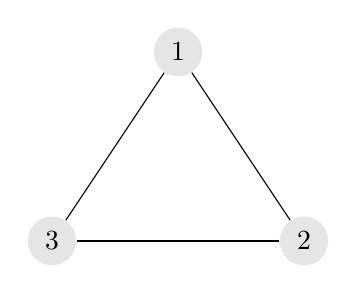
\begin{tikzpicture}
  [scale=.8,auto=left,every node/.style={circle,fill=gray!20}]
  \node (n1) at (5,5) {1};
  \node (n2) at (7,2)  {2};
  \node (n3) at (3,2)  {3};

  \foreach \from/\to in {n1/n2,n1/n3,n2/n3}
    \draw (\from) -- (\to);
\end{tikzpicture}
\caption{A network of three peers}
\label{fig:threepeers}
\end{figure}


\subparagraph{Firewall Problems}
In a test having one process running on a server in Internet and outside of the local network and having two
different processes running on one laptop but on different ports it is observed that the changes (sets) in the
Internet does not replicate to the local processes but the changes from local processes are being replicated to the other process.

\subparagraph{conclusion}
Having a network between local and Internet processes in the above mentioned method is not reliable. 
Repeating the tests with only local processes which are bootstrapping to one of them and running the setter/getter
methods showed that even in this scenario it is not reliable and one can not guarantee that the desired value will be returned.


\subsection{Concoord}
Describe why it is not suitable for us. It allows single object sharing.

\section{Distributed Workflows}
In this section we introduce a number of existing scientific workflow systems.
\subsection{COSMOS}\cite{Gafni30062014}
\subsection{Weaver}\cite{Bui_weaver:integrating}
\chapter{Scenarios}
\label{cha:scenarios}

There are a number of possible use cases in our problem domain. To demonstrate these cases we assume
we have a number of nodes and datasets respectively, but they are not necessarily on the same nodes.
In the following paragraphs we explain possible combinations of operations, nodes and datasets.

\section{Operation}
In every scenario we want to run an operation which could be linear or non-linear.

\subsection{Linear Operation}
Being linear means that the operation
could be broken into its components and then run in parallel or series. Here is algebic notation
of a linear operation which acts on two datasets:

\[ Operation(A + B) = Operation(A) + Operation(B) \]

Being linear or non-linear only matters when we have to operate on more that one dataset.

\subsection{Non-linear Operation}
In contrast to linear there is non-linear operation. This means that this kind of operation has dependant parts and
those parts could not run in parallel:

\[ Operation(A + B) \neq Operation(A) + Operation(B) \]

\section{Datasets}
For each operation we need one or more datasets which my be available on the same node that wants to run the operation
initially or could reside on other nodes. 

\subsection{Input}
Input files are normally not mission critical and could be reproduced.

\subsection{Output}
Operations create output datasets which normally are small in size, threfore we ignore the transfer cost of operation
results in our work.

\subsection{Data Locationing}
We consider three different approaches toward preparing required data for operations.
\subsubsection{Conventional Approach}
in this approach we put the required data on a network file system and all
application instances will access it there. We will utilize an NFS mounted file system.
\subsubsection{Centralized Approach}
in this approach we will have a central instance which will orchestrate operation
delegation and operation output forwarding to other nodes.
\subsubsection{Decentralized Approach}
in this approach we will eliminate the orchestrator node and the network of
application instances should collaborate in a decentralized fashion to keep track of data and control flow for each
task.

For every approach we will run performance tests and we will compare the results.

\subsubsection{Method}
We will discuss scenarios in chapter\ref{cha:scenarios}. For each scenario we will analyze the possible combinations 
of data and operations and we will discuss how to 
deliver the input data and where to store output data. We will discuss workflow management in chapter 
\ref{cha:workflow} and data transfer in chapter\ref{cha:data}.


% TODO: I might need to introduce "Decision Tree"
\section{Decision Making}
The main decision that we need to make at every scenario is whether we should transfer the required data or we
need to delegate the operation to an instance on a node which already has the data. To make a decision we need to
answer a number of questions. First we need to know the location of the data:

\begin{enumerate}
\item Is the data available locally?
\item If not, is the data available on another node? -- Here only the physical location of data matters not the instance
controlling it.
\end{enumerate}

% TODO: Introduce "Decision Metrics"

%In case the mentioned data is available on another nodes we have to answer these questions:
%\begin{enumerate}
%\item What is the cost of data transfer? -- We have to invent an algorithm for this calculation
%\item If data is available on more than one remote node, which one has the minimum transfer cost? -- We might
%introduce multiple strategies and use some heuristics for this selection, simplest form would be random selection,
%another could be asking for an availability metric from the instance and mix it with local calculated availability 
%metric to get a final cost value.
% TODO: We can use "Heartbeat" concept as one of availability metrics
%\item In case it is expensive to transfer the data, can we delegate the operation to an instance on the other node?
%\end{enumerate}



\section{Concrete Scenarios}
We begin with a simple scenario and we gradually add details to it and build new scenarios.

\subsection{Scenario 1}
In this scenario we have a linear operation, e.g. \(Op^A\) on \(Node^A\) which
requires one single dataset such as \( Dataset^1 \) which is available on one of the other peers.

\subsubsection{Conditions} \( Dataset^1 \) is not available on \( Node^A \) and the operation is linear.
\subsubsection{Consequences} With these conditions we either should transfer \( Dataset^1 \)
to local node or in case of availability delegate \(Op^A\) to the node which already has \( Dataset^1 \).

\subsection{Use Case Description}
We have a distributed network of collaborating servers, where in this case, we consider two computers. 
Each server has its own storage and maintains a number of datasets on it. These servers collaborate 
together to accomplish issued commands. User in this case wants to perform one operation on a dataset
that resides only on one of the servers. There are two main assumptions here:
\begin{enumerate}
\item \textbf{The user has neighter a prior knowledge where the data is stored}
\item \textbf{Nor of how many servers are present on the network}
\end{enumerate}

The user connects to one of the servers, which we call a client. This server is assumed to be part 
of the network, though it may not have any local data stores on it. The user issues, interactively
(or non-interactively) a command on a set of data providing some kind of identification. This command
is broadcasted by the client to all servers in the network. All servers receive this command and check
whether they have the data locally. The server which has the data performs the operation and the others
ignore it. The result of the operation in this case, remains on the same server which the original 
dataset was on. 

\begin{itemize}
\item Note: it is assumed that at any instance of time, only one server acts as a client.
\end{itemize}

Moreover we assume the user has already queried the available data in the entire network by 
issueing something like “list datasets” which outputs dataset names and ids.

The following table shows two servers, each has one dataset. The user is connected to S2.\\

\begin{tabular}{ l c r }
\em{Server ID} & \em{ Dataset ID} & \em{ Client} \\
S1 & DS1 & No \\
S2 & DS2 & Yes \\
\end{tabular}\\

Let us assume the data sets are \(10^6\) random numbers.
Let us assume the operation is to transform the real random numbers to a set of [0 or 1 ] depending on whether the number is even or odd. 
This operation is assumed here to be a user defined method that operates on the data set.

\begin{itemize}
\item Note: A dataset can be for example defined as an object that has an id, and a one dimensional array (python list).
\end{itemize}

The user issues the command like this from a python shell: 

\begin{itemize}
\item real2bin(DS1) will result in -> Broadcast(real2bin(DS1))
\item Note: it is assumed that all functions are already defined on all servers, since they execute the same environment.
\end{itemize}

The client broadcasts this function to all servers. Each server will check if the data set with this id exists, if so will run the command. 

This means that each server, especially the client, has to “know about all data sets existing in all servers.
It does not need to have the actual data, but needs to know about it. So that when the user issues the command
above, he/she does not get a “data structure not existent” error from the client, just because the data is not
there. Hence we need some interface, or some wrapper function that checks the argument for the data type, or to 
create some proxy interface from all data to all nodes. 

\section{Assessing Suggested Approaches}
To be able to assess the performance of each given solution to the mentioned scenarios we made a demo application
called \testbf{Konsensus}. The code is available on Github. %TODO add ref here

\subsection{Testing Problems}
Writing tests for a distributed application is not as easy as writing unittests for a normal application. 
Our demo application acts as a server and client at the same time. Moreover we want to launch multiple 
network peers running on one or multiple machines. Testing scenarios on this network is not possible with
normal mocking approaches, because we need to test the behaviour of our solution in a network of collaborating
peers which are not external services, rather the core services of the application.

To overcome testing issues we have to launch the desired number of peers separately and then run our tests 
over them. To make this operation faster we changed the application to make it possible to launch any number
of instances on one machine and we automated this process using a number of scripts. %TODO more details

\subsubsection{Mixing Signals in Greenlets}
We use python Greenlets instead of threads. This means that our demo application runs on only one thread. 
This causes a problem when launching multiple apps all together with one script and inside one thread, that
causes the signals for events spread among all greenlets and make trouble. To avoid this we have to run
each server in a separate processes. Running them inside threads won't help as well because the blinker python
library is threadsafe so it moves signals between threads as well as greenlets.
\chapter{Workflow Management}
\label{cha:workflow}
\chapter{Data Transfer}
\label{cha:data}

%\appendix % The Proposal

\printbibliography[heading=bibintoc, title={References}]

\end{document}